\documentclass[12pt, letterpaper]{article}
\usepackage{hyperref}
\hypersetup{
    colorlinks,
    citecolor=blue,
    filecolor=black,
    linkcolor=red,
    urlcolor={medium-blue},
    hypertexnames=false
}
\usepackage[margin=1in]{geometry}
\usepackage{amsmath}
\usepackage{mathtools}
\usepackage{amssymb}
\usepackage{amsthm}
\usepackage{fancyhdr}
\usepackage{booktabs}
\usepackage[inline]{enumitem}
\usepackage{amsfonts}
\usepackage{textcomp}
\usepackage{tabularx}
\usepackage{pgfplots}
\usepackage{bm}
\usepackage{float}
\usepackage{tabto}
\usepackage{clrscode3e}
\usepackage{textcomp}
\usepackage{graphics}
\usepackage{graphicx}
\usepackage{listings, xcolor}
\pgfplotsset{compat=newest}
\usepackage{tikz}
\author{Specification Group}
\title{CISC 3140 SyRS}
\pagestyle{fancy}
\renewcommand{\headrulewidth}{0pt}
\renewcommand{\footrulewidth}{0pt}
\renewcommand{\qedsymbol}{$\blacksquare$}
\newbox\fixbox
\DeclarePairedDelimiter\abs{\lvert}{\rvert}
\renewenvironment{proof}{{\bfseries Proof.}}{\hfill\qedsymbol}
\DeclarePairedDelimiter\ceil{\lceil}{\rceil}
\DeclarePairedDelimiter\floor{\lfloor}{\rfloor}
\usepackage[all]{hypcap}
\setcounter{tocdepth}{3}
\setcounter{secnumdepth}{3}
\definecolor{medium-blue}{rgb}{0,0,1}


\graphicspath{ {./images/} }

\headheight = 41.55003pt

\fancyhf{}
\lhead{CISC 3140 SyRS\\
       Version 3.7.2022.1\\}
       
\rfoot{Page \thepage}
\begin{document}
   \centerline{\textbf{System Requirements Specification}}
   \centerline{\textbf{for Space Invader Game}}
   
   \tableofcontents
    
    \newpage{}
    
   \vspace{50px}
   
   
   \section{Introduction}
   
   \noindent This SyRS is written for the CISC 3140 semester project at Brooklyn College. This document is a work-in-progress, so nothing is concrete. The game is supposed to be a working copy of the famous game \textit{Space Invaders}\footnote{\href{https://en.wikipedia.org/wiki/Space_Invaders}{https://en.wikipedia.org/wiki/Space\_Invaders}}. Here is what the game looks like for those that are not familiar:
       
   \label{gamepic}
   \vspace{10px}
   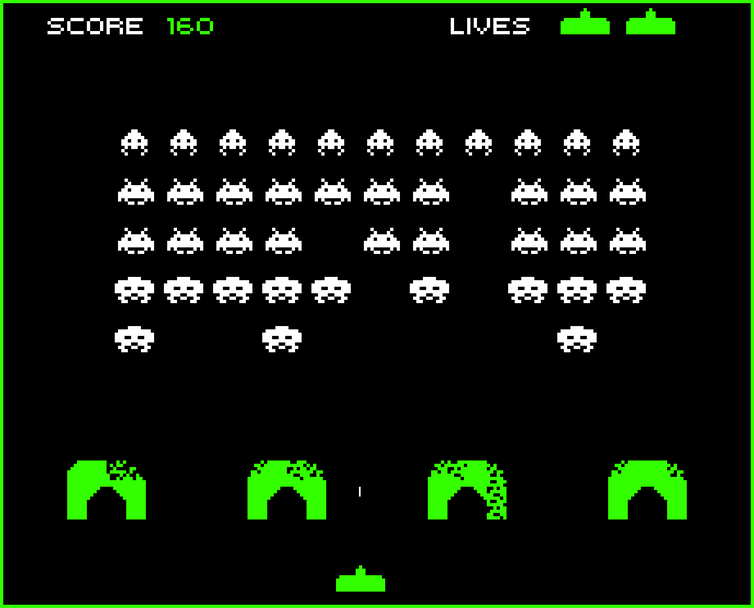
\includegraphics[scale=0.5]{si}
   \vspace{10px}
    

    \noindent To add our own twist on the game, instead of the aliens being enemies we will have City University of New York's Deans and Trustees, the spaceship will be the student, and the space bases will be the Professors, so the Brooklyn College professors will shield the students from the evil Deans and Trustees. A more detailed description will be given in later sections. 
   
   \section{Basic Software Expectations}
   
   Here we list requirements the Software must meet. 
   
   \phantomsection
   \addcontentsline{toc}{subsection}{BSR.1}
   \subsection*{BSR.1}
   
    The game should run smoothly (without any blatant bugs/software issues due to the developer) provided that the user has the required hardware to run the game.
    \begin{enumerate}[label=]
        \phantomsection
        \addcontentsline{toc}{subsubsection}{BSR.1.1}
        \subsubsection*{BSR.1.1}
        \item If the user's hardware is capable, the game should be able to run at 60 fps or higher.
        \phantomsection
        \addcontentsline{toc}{subsubsection}{BSR.2.2}
        \subsubsection*{BSR.2.2}
        \item The game should be able to read the user's inputs without too much of a delay. For example, if I move the spaceship to the right, there should be no noticeable delay. 
    \end{enumerate}
    
    \phantomsection
    \addcontentsline{toc}{subsection}{BSR.2}
    \subsection*{BSR.2}
    
    The game should run on multiple browsers/hardware.
    \begin{enumerate}[label=]
        \phantomsection
        \addcontentsline{toc}{subsubsection}{BSR.2.1}
        \subsubsection*{BSR.2.1}
        \item Game must run on both the PC and Mobile versions of Google Chrome, Firefox, and Safari.
    \end{enumerate}
    
    
    
    \section{Game Expectations}
    
    As mentioned in the introduction, the game should be a replica of Space Invaders. We will now list some requirements the game must meet. 
    
    \phantomsection
    \addcontentsline{toc}{subsection}{GR.1}
    \subsection*{GR.1}
    
    Like the original game, there must be a `start' screen that is displayed to the user upon loading the game. 
    
    \begin{enumerate}[label=]
        \phantomsection
        \addcontentsline{toc}{subsubsection}{GR.1.1}
        \subsubsection*{GR.1.1}
        \item The start screen will display the name of the game. We have not yet decided on the title for the game, but it will be displayed in big bold font. 
        \phantomsection
        \addcontentsline{toc}{subsubsection}{GR.1.2}
        \subsubsection*{GR.1.2}
        \label{aliens}
        \item Below the game title, the start screen should show the different types of aliens and the number of points each alien rewards when it dies. In our twist there will be no aliens---instead, there will be deans and trustees. We have not yet decided which dean or trustee will be displayed. Perhaps we can generate them randomly when the game loads, or we can allow the user to choose the deans and trustees they want to fight. 
        \phantomsection
        \addcontentsline{toc}{subsubsection}{GR.1.3}
        \subsubsection*{GR.1.3}
        \label{play_again}
        \item Below the deans and trustees there will be a text saying \verb#PRESS ANY KEY TO BEGIN# telling the user that the game needs to be started by providing an input. We will want this text to be dynamic---that is, it will grow and shrink to get the user's attention. 
        \phantomsection
        \addcontentsline{toc}{subsubsection}{GR.1.4}
        \subsubsection*{GR.1.4}
        \item Finally, below the flashing text we will have the default keys and their function. We will have a picture of the arrow keys along with an equal sign saying that the keys are used for movement, and a picture of the space bar with an equal sign followed by ``shoot'', telling the user that the space bar is used to shoot. Of course these controls are for PCs, so we will have to display something alternate for mobile users. For mobile users, we will show two animated images. The first animated image will show a hand holding a phone and the hand's thumb will be sliding horizontally across the bottom of the screen with an equal sign followed by ``movement''. Another animated image will show the thumb tapping the screen followed by an equal sign saying ``shoot''.
    \end{enumerate}
    
    \phantomsection
    \addcontentsline{toc}{subsection}{GR.2}
    \subsection*{GR.2}
    
    Once the user provides an input on the start screen, the main game will begin. We will now list some expectations of the main game. 
    \begin{enumerate}[label=]
        \phantomsection
        \addcontentsline{toc}{subsubsection}{GR.2.1}
        \subsubsection*{GR.2.1}
        \item When the game begins, we will show a short cinematic. The cinematic will just be a dialogue box that says ``The evil Deans and Trustees of CUNY have come to attack the students. Help defend the students from the Dean and Trustee barrage!". The text will not be displayed all at once. It will be displayed one word at a time. The rate at which each word is displayed has not yet been decided. We will then show the 4 evil Deans and Trustees from \nameref{aliens}.
        \phantomsection
        \addcontentsline{toc}{subsubsection}{GR.2.2}
        \subsubsection*{GR.2.2}
        \item Once the cinematic has finished, we will officially begin the game. We will now discuss the elements of the game. The game will be divided into three areas. See \nameref{fig:game_rect} on next page.
        
        
        \begin{figure}[!htb]
        \begin{center}
        \begin{tikzpicture}
            \draw[blue] (0,-2) rectangle (15.5,0);
            \draw[red]  (0,-2) rectangle (15.5, -8);
            \draw[green] (0, -8) rectangle (15.5, -12);
        \end{tikzpicture}
        \caption{Game Rectangle}
        \label{fig:game_rect}
        \end{center}
        \end{figure}
        \phantomsection
        \addcontentsline{toc}{subsubsection}{GR.2.3}
        \subsubsection*{GR.2.3}
        \item The blue rectangle, the rectangle on top, will display the player's score and the number of lives the player has. In the left corner of this rectangle will be the player's score. It will be displayed exactly like the picture in the \nameref{gamepic}. Similarly, the right corner of this rectangle should display the number of lives the player has. 
        \phantomsection
        \addcontentsline{toc}{subsubsection}{GR.2.4}
        \subsubsection*{GR.2.4}
        \label{enemy_rect}
        \item The red rectangle, the second rectangle, will contain the enemies. See \nameref{fig:enemy_rect} for more detail.
        \begin{figure}[H]
        \begin{center}
        \begin{tikzpicture}
            \draw[red]  (0,2) rectangle (15.5, 8);
            \draw[red]  (0 + 15*15.5/40, 7) rectangle (0 + 16*15.5/40, 6.5);
            \draw[red]  (0 + 16*15.5/40, 7) rectangle (0 + 17*15.5/40, 6.5);
            \draw[red]  (0 + 17*15.5/40, 7) rectangle (0 + 18*15.5/40, 6.5);
            \draw[red]  (0 + 18*15.5/40, 7) rectangle (0 + 19*15.5/40, 6.5);
            \draw[red]  (0 + 19*15.5/40, 7) rectangle (0 + 20*15.5/40, 6.5);
            \draw[red]  (0 + 20*15.5/40, 7) rectangle (0 + 21*15.5/40, 6.5);
            \draw[red]  (0 + 21*15.5/40, 7) rectangle (0 + 22*15.5/40, 6.5);
            \draw[red]  (0 + 22*15.5/40, 7) rectangle (0 + 23*15.5/40, 6.5);
            \draw[red]  (0 + 23*15.5/40, 7) rectangle (0 + 24*15.5/40, 6.5);
            \draw[red]  (0 + 24*15.5/40, 7) rectangle (0 + 25*15.5/40, 6.5);
            \draw[red]  (0 + 25*15.5/40, 7) rectangle (0 + 26*15.5/40, 6.5);
            \draw[blue]  (0 + 15*15.5/40, 6.5) rectangle (0 + 16*15.5/40, 6);
            \draw[blue]  (0 + 16*15.5/40, 6.5) rectangle (0 + 17*15.5/40, 6);
            \draw[blue]  (0 + 17*15.5/40, 6.5) rectangle (0 + 18*15.5/40, 6);
            \draw[blue]  (0 + 18*15.5/40, 6.5) rectangle (0 + 19*15.5/40, 6);
            \draw[blue]  (0 + 19*15.5/40, 6.5) rectangle (0 + 20*15.5/40, 6);
            \draw[blue]  (0 + 20*15.5/40, 6.5) rectangle (0 + 21*15.5/40, 6);
            \draw[blue]  (0 + 21*15.5/40, 6.5) rectangle (0 + 22*15.5/40, 6);
            \draw[blue]  (0 + 22*15.5/40, 6.5) rectangle (0 + 23*15.5/40, 6);
            \draw[blue]  (0 + 23*15.5/40, 6.5) rectangle (0 + 24*15.5/40, 6);
            \draw[blue]  (0 + 24*15.5/40, 6.5) rectangle (0 + 25*15.5/40, 6);
            \draw[blue]  (0 + 25*15.5/40, 6.5) rectangle (0 + 26*15.5/40, 6);
            \draw[blue]  (0 + 15*15.5/40, 6) rectangle (0 + 16*15.5/40, 5.5);
            \draw[blue]  (0 + 16*15.5/40, 6) rectangle (0 + 17*15.5/40, 5.5);
            \draw[blue]  (0 + 17*15.5/40, 6) rectangle (0 + 18*15.5/40, 5.5);
            \draw[blue]  (0 + 18*15.5/40, 6) rectangle (0 + 19*15.5/40, 5.5);
            \draw[blue]  (0 + 19*15.5/40, 6) rectangle (0 + 20*15.5/40, 5.5);
            \draw[blue]  (0 + 20*15.5/40, 6) rectangle (0 + 21*15.5/40, 5.5);
            \draw[blue]  (0 + 21*15.5/40, 6) rectangle (0 + 22*15.5/40, 5.5);
            \draw[blue]  (0 + 22*15.5/40, 6) rectangle (0 + 23*15.5/40, 5.5);
            \draw[blue]  (0 + 23*15.5/40, 6) rectangle (0 + 24*15.5/40, 5.5);
            \draw[blue]  (0 + 24*15.5/40, 6) rectangle (0 + 25*15.5/40, 5.5);
            \draw[blue]  (0 + 25*15.5/40, 6) rectangle (0 + 26*15.5/40, 5.5);
            
            \draw[magenta]  (0 + 15*15.5/40, 5.5) rectangle (0 + 16*15.5/40, 5);
            \draw[magenta]  (0 + 16*15.5/40, 5.5) rectangle (0 + 17*15.5/40, 5);
            \draw[magenta]  (0 + 17*15.5/40, 5.5) rectangle (0 + 18*15.5/40, 5);
            \draw[magenta]  (0 + 18*15.5/40, 5.5) rectangle (0 + 19*15.5/40, 5);
            \draw[magenta]  (0 + 19*15.5/40, 5.5) rectangle (0 + 20*15.5/40, 5);
            \draw[magenta]  (0 + 20*15.5/40, 5.5) rectangle (0 + 21*15.5/40, 5);
            \draw[magenta]  (0 + 21*15.5/40, 5.5) rectangle (0 + 22*15.5/40, 5);
            \draw[magenta]  (0 + 22*15.5/40, 5.5) rectangle (0 + 23*15.5/40, 5);
            \draw[magenta]  (0 + 23*15.5/40, 5.5) rectangle (0 + 24*15.5/40, 5);
            \draw[magenta]  (0 + 24*15.5/40, 5.5) rectangle (0 + 25*15.5/40, 5);
            \draw[magenta]  (0 + 25*15.5/40, 5.5) rectangle (0 + 26*15.5/40, 5);
            
            \draw[magenta]  (0 + 15*15.5/40, 5) rectangle (0 + 16*15.5/40, 4.5);
            \draw[magenta]  (0 + 16*15.5/40, 5) rectangle (0 + 17*15.5/40, 4.5);
            \draw[magenta]  (0 + 17*15.5/40, 5) rectangle (0 + 18*15.5/40, 4.5);
            \draw[magenta]  (0 + 18*15.5/40, 5) rectangle (0 + 19*15.5/40, 4.5);
            \draw[magenta]  (0 + 19*15.5/40, 5) rectangle (0 + 20*15.5/40, 4.5);
            \draw[magenta]  (0 + 20*15.5/40, 5) rectangle (0 + 21*15.5/40, 4.5);
            \draw[magenta]  (0 + 21*15.5/40, 5) rectangle (0 + 22*15.5/40, 4.5);
            \draw[magenta]  (0 + 22*15.5/40, 5) rectangle (0 + 23*15.5/40, 4.5);
            \draw[magenta]  (0 + 23*15.5/40, 5) rectangle (0 + 24*15.5/40, 4.5);
            \draw[magenta]  (0 + 24*15.5/40, 5) rectangle (0 + 25*15.5/40, 4.5);
            \draw[magenta]  (0 + 25*15.5/40, 5) rectangle (0 + 26*15.5/40, 4.5);
        \end{tikzpicture}
        \caption{Enemy Rectangle}
        \label{fig:enemy_rect}
        \end{center}
        \end{figure}
        As you can see by the different colors of the small rectangles, there will be 3 types of enemies as mentioned in \nameref{aliens}. Killing the enemy denoted by the small rectangle will reward 40 points, killing the enemy denoted by the small blue rectangles will reward 20 points, and killing the enemy denoted by the small magenta rectangles will reward 10 points. The enemies will move across the red rectangle until they reach the end of the rectangle. When the aliens reach the following position: 
         \begin{figure}[H]
        \begin{center}
        \begin{tikzpicture}
            \draw[red]  (0,2) rectangle (15.5, 8);
            \draw[red]  (0 + 29*15.5/40, 7) rectangle (0 + 30*15.5/40, 6.5);
            \draw[red]  (0 + 30*15.5/40, 7) rectangle (0 + 31*15.5/40, 6.5);
            \draw[red]  (0 + 31*15.5/40, 7) rectangle (0 + 32*15.5/40, 6.5);
            \draw[red]  (0 + 32*15.5/40, 7) rectangle (0 + 33*15.5/40, 6.5);
            \draw[red]  (0 + 33*15.5/40, 7) rectangle (0 + 34*15.5/40, 6.5);
            \draw[red]  (0 + 34*15.5/40, 7) rectangle (0 + 35*15.5/40, 6.5);
            \draw[red]  (0 + 35*15.5/40, 7) rectangle (0 + 36*15.5/40, 6.5);
            \draw[red]  (0 + 36*15.5/40, 7) rectangle (0 + 37*15.5/40, 6.5);
            \draw[red]  (0 + 37*15.5/40, 7) rectangle (0 + 38*15.5/40, 6.5);
            \draw[red]  (0 + 38*15.5/40, 7) rectangle (0 + 39*15.5/40, 6.5);
            \draw[red]  (0 + 39*15.5/40, 7) rectangle (0 + 40*15.5/40, 6.5);
            
            \draw[blue]  (0 + 29*15.5/40, 6.5) rectangle (0 + 30*15.5/40, 6);
            \draw[blue]  (0 + 30*15.5/40, 6.5) rectangle (0 + 31*15.5/40, 6);
            \draw[blue]  (0 + 31*15.5/40, 6.5) rectangle (0 + 32*15.5/40, 6);
            \draw[blue]  (0 + 32*15.5/40, 6.5) rectangle (0 + 33*15.5/40, 6);
            \draw[blue]  (0 + 33*15.5/40, 6.5) rectangle (0 + 34*15.5/40, 6);
            \draw[blue]  (0 + 34*15.5/40, 6.5) rectangle (0 + 35*15.5/40, 6);
            \draw[blue]  (0 + 35*15.5/40, 6.5) rectangle (0 + 36*15.5/40, 6);
            \draw[blue]  (0 + 36*15.5/40, 6.5) rectangle (0 + 37*15.5/40, 6);
            \draw[blue]  (0 + 37*15.5/40, 6.5) rectangle (0 + 38*15.5/40, 6);
            \draw[blue]  (0 + 38*15.5/40, 6.5) rectangle (0 + 39*15.5/40, 6);
            \draw[blue]  (0 + 39*15.5/40, 6.5) rectangle (0 + 40*15.5/40, 6);
            
            \draw[blue]  (0 + 29*15.5/40, 6) rectangle (0 + 30*15.5/40, 5.5);
            \draw[blue]  (0 + 30*15.5/40, 6) rectangle (0 + 31*15.5/40, 5.5);
            \draw[blue]  (0 + 31*15.5/40, 6) rectangle (0 + 32*15.5/40, 5.5);
            \draw[blue]  (0 + 32*15.5/40, 6) rectangle (0 + 33*15.5/40, 5.5);
            \draw[blue]  (0 + 33*15.5/40, 6) rectangle (0 + 34*15.5/40, 5.5);
            \draw[blue]  (0 + 34*15.5/40, 6) rectangle (0 + 35*15.5/40, 5.5);
            \draw[blue]  (0 + 35*15.5/40, 6) rectangle (0 + 36*15.5/40, 5.5);
            \draw[blue]  (0 + 36*15.5/40, 6) rectangle (0 + 37*15.5/40, 5.5);
            \draw[blue]  (0 + 37*15.5/40, 6) rectangle (0 + 38*15.5/40, 5.5);
            \draw[blue]  (0 + 38*15.5/40, 6) rectangle (0 + 39*15.5/40, 5.5);
            \draw[blue]  (0 + 39*15.5/40, 6) rectangle (0 + 40*15.5/40, 5.5);
            
            \draw[magenta]  (0 + 29*15.5/40, 5.5) rectangle (0 + 30*15.5/40, 5);
            \draw[magenta]  (0 + 30*15.5/40, 5.5) rectangle (0 + 31*15.5/40, 5);
            \draw[magenta]  (0 + 31*15.5/40, 5.5) rectangle (0 + 32*15.5/40, 5);
            \draw[magenta]  (0 + 32*15.5/40, 5.5) rectangle (0 + 33*15.5/40, 5);
            \draw[magenta]  (0 + 33*15.5/40, 5.5) rectangle (0 + 34*15.5/40, 5);
            \draw[magenta]  (0 + 34*15.5/40, 5.5) rectangle (0 + 35*15.5/40, 5);
            \draw[magenta]  (0 + 35*15.5/40, 5.5) rectangle (0 + 36*15.5/40, 5);
            \draw[magenta]  (0 + 36*15.5/40, 5.5) rectangle (0 + 37*15.5/40, 5);
            \draw[magenta]  (0 + 37*15.5/40, 5.5) rectangle (0 + 38*15.5/40, 5);
            \draw[magenta]  (0 + 38*15.5/40, 5.5) rectangle (0 + 39*15.5/40, 5);
            \draw[magenta]  (0 + 39*15.5/40, 5.5) rectangle (0 + 40*15.5/40, 5);
            
            \draw[magenta]  (0 + 29*15.5/40, 5) rectangle (0 + 30*15.5/40, 4.5);
            \draw[magenta]  (0 + 30*15.5/40, 5) rectangle (0 + 31*15.5/40, 4.5);
            \draw[magenta]  (0 + 31*15.5/40, 5) rectangle (0 + 32*15.5/40, 4.5);
            \draw[magenta]  (0 + 32*15.5/40, 5) rectangle (0 + 33*15.5/40, 4.5);
            \draw[magenta]  (0 + 33*15.5/40, 5) rectangle (0 + 34*15.5/40, 4.5);
            \draw[magenta]  (0 + 34*15.5/40, 5) rectangle (0 + 35*15.5/40, 4.5);
            \draw[magenta]  (0 + 35*15.5/40, 5) rectangle (0 + 36*15.5/40, 4.5);
            \draw[magenta]  (0 + 36*15.5/40, 5) rectangle (0 + 37*15.5/40, 4.5);
            \draw[magenta]  (0 + 37*15.5/40, 5) rectangle (0 + 38*15.5/40, 4.5);
            \draw[magenta]  (0 + 38*15.5/40, 5) rectangle (0 + 39*15.5/40, 4.5);
            \draw[magenta]  (0 + 39*15.5/40, 5) rectangle (0 + 40*15.5/40, 4.5);
        \end{tikzpicture}
        \caption{Enemies Reach Border}
        \label{fig:enemy_end}
        \end{center}
        \end{figure}
        The enemies will move down vertically: 
         \begin{figure}[H]
        \begin{center}
        \begin{tikzpicture}
            \draw[red]  (0,2) rectangle (15.5, 8);
            \draw[red]  (0 + 29*15.5/40, 6.5) rectangle (0 + 30*15.5/40, 6);
            \draw[red]  (0 + 30*15.5/40, 6.5) rectangle (0 + 31*15.5/40, 6);
            \draw[red]  (0 + 31*15.5/40, 6.5) rectangle (0 + 32*15.5/40, 6);
            \draw[red]  (0 + 32*15.5/40, 6.5) rectangle (0 + 33*15.5/40, 6);
            \draw[red]  (0 + 33*15.5/40, 6.5) rectangle (0 + 34*15.5/40, 6);
            \draw[red]  (0 + 34*15.5/40, 6.5) rectangle (0 + 35*15.5/40, 6);
            \draw[red]  (0 + 35*15.5/40, 6.5) rectangle (0 + 36*15.5/40, 6);
            \draw[red]  (0 + 36*15.5/40, 6.5) rectangle (0 + 37*15.5/40, 6);
            \draw[red]  (0 + 37*15.5/40, 6.5) rectangle (0 + 38*15.5/40, 6);
            \draw[red]  (0 + 38*15.5/40, 6.5) rectangle (0 + 39*15.5/40, 6);
            \draw[red]  (0 + 39*15.5/40, 6.5) rectangle (0 + 40*15.5/40, 6);
            
            \draw[blue]  (0 + 29*15.5/40, 6) rectangle (0 + 30*15.5/40, 5.5);
            \draw[blue]  (0 + 30*15.5/40, 6) rectangle (0 + 31*15.5/40, 5.5);
            \draw[blue]  (0 + 31*15.5/40, 6) rectangle (0 + 32*15.5/40, 5.5);
            \draw[blue]  (0 + 32*15.5/40, 6) rectangle (0 + 33*15.5/40, 5.5);
            \draw[blue]  (0 + 33*15.5/40, 6) rectangle (0 + 34*15.5/40, 5.5);
            \draw[blue]  (0 + 34*15.5/40, 6) rectangle (0 + 35*15.5/40, 5.5);
            \draw[blue]  (0 + 35*15.5/40, 6) rectangle (0 + 36*15.5/40, 5.5);
            \draw[blue]  (0 + 36*15.5/40, 6) rectangle (0 + 37*15.5/40, 5.5);
            \draw[blue]  (0 + 37*15.5/40, 6) rectangle (0 + 38*15.5/40, 5.5);
            \draw[blue]  (0 + 38*15.5/40, 6) rectangle (0 + 39*15.5/40, 5.5);
            \draw[blue]  (0 + 39*15.5/40, 6) rectangle (0 + 40*15.5/40, 5.5);
            
            \draw[blue]  (0 + 29*15.5/40, 5.5) rectangle (0 + 30*15.5/40, 5);
            \draw[blue]  (0 + 30*15.5/40, 5.5) rectangle (0 + 31*15.5/40, 5);
            \draw[blue]  (0 + 31*15.5/40, 5.5) rectangle (0 + 32*15.5/40, 5);
            \draw[blue]  (0 + 32*15.5/40, 5.5) rectangle (0 + 33*15.5/40, 5);
            \draw[blue]  (0 + 33*15.5/40, 5.5) rectangle (0 + 34*15.5/40, 5);
            \draw[blue]  (0 + 34*15.5/40, 5.5) rectangle (0 + 35*15.5/40, 5);
            \draw[blue]  (0 + 35*15.5/40, 5.5) rectangle (0 + 36*15.5/40, 5);
            \draw[blue]  (0 + 36*15.5/40, 5.5) rectangle (0 + 37*15.5/40, 5);
            \draw[blue]  (0 + 37*15.5/40, 5.5) rectangle (0 + 38*15.5/40, 5);
            \draw[blue]  (0 + 38*15.5/40, 5.5) rectangle (0 + 39*15.5/40, 5);
            \draw[blue]  (0 + 39*15.5/40, 5.5) rectangle (0 + 40*15.5/40, 5);
            
            \draw[magenta]  (0 + 29*15.5/40, 5) rectangle (0 + 30*15.5/40, 4.5);
            \draw[magenta]  (0 + 30*15.5/40, 5) rectangle (0 + 31*15.5/40, 4.5);
            \draw[magenta]  (0 + 31*15.5/40, 5) rectangle (0 + 32*15.5/40, 4.5);
            \draw[magenta]  (0 + 32*15.5/40, 5) rectangle (0 + 33*15.5/40, 4.5);
            \draw[magenta]  (0 + 33*15.5/40, 5) rectangle (0 + 34*15.5/40, 4.5);
            \draw[magenta]  (0 + 34*15.5/40, 5) rectangle (0 + 35*15.5/40, 4.5);
            \draw[magenta]  (0 + 35*15.5/40, 5) rectangle (0 + 36*15.5/40, 4.5);
            \draw[magenta]  (0 + 36*15.5/40, 5) rectangle (0 + 37*15.5/40, 4.5);
            \draw[magenta]  (0 + 37*15.5/40, 5) rectangle (0 + 38*15.5/40, 4.5);
            \draw[magenta]  (0 + 38*15.5/40, 5) rectangle (0 + 39*15.5/40, 4.5);
            \draw[magenta]  (0 + 39*15.5/40, 5) rectangle (0 + 40*15.5/40, 4.5);
            
            \draw[magenta]  (0 + 29*15.5/40, 4.5) rectangle (0 + 30*15.5/40, 4);
            \draw[magenta]  (0 + 30*15.5/40, 4.5) rectangle (0 + 31*15.5/40, 4);
            \draw[magenta]  (0 + 31*15.5/40, 4.5) rectangle (0 + 32*15.5/40, 4);
            \draw[magenta]  (0 + 32*15.5/40, 4.5) rectangle (0 + 33*15.5/40, 4);
            \draw[magenta]  (0 + 33*15.5/40, 4.5) rectangle (0 + 34*15.5/40, 4);
            \draw[magenta]  (0 + 34*15.5/40, 4.5) rectangle (0 + 35*15.5/40, 4);
            \draw[magenta]  (0 + 35*15.5/40, 4.5) rectangle (0 + 36*15.5/40, 4);
            \draw[magenta]  (0 + 36*15.5/40, 4.5) rectangle (0 + 37*15.5/40, 4);
            \draw[magenta]  (0 + 37*15.5/40, 4.5) rectangle (0 + 38*15.5/40, 4);
            \draw[magenta]  (0 + 38*15.5/40, 4.5) rectangle (0 + 39*15.5/40, 4);
            \draw[magenta]  (0 + 39*15.5/40, 4.5) rectangle (0 + 40*15.5/40, 4);
        \end{tikzpicture}
        \caption{Enemies Move Down}
        \label{fig:enemy_down}
        \end{center}
        \end{figure}
        Then the enemies will continue moving horizontally to the left until they reach a position analogous to \nameref{fig:enemy_end} in which case the enemies will move down vertically analogously to \nameref{fig:enemy_down}. This process will repeat until the enemies reach the green rectangle from \nameref{fig:game_rect}; if an enemy is in the green rectangle, the game ends and the player loses. 
        \phantomsection
        \addcontentsline{toc}{subsubsection}{GR.2.5}
        \subsubsection*{GR.2.5}
        \item Now we discuss the speed at which the aliens move. The aliens will begin the game by moving once every second. The number of times the aliens move per second will scale with time. For every second that passes, the number of times the aliens move per second will be increase by $0.1.$ For example, say that 10 seconds have elapsed since the game started: the aliens should move twice every second, and if 25 seconds have elapsed, the aliens should move 3.5 times every second---but since 3.5 movements per second does not make sense, we will floor the number to get 3 movements per second. 
        \phantomsection
        \addcontentsline{toc}{subsubsection}{GR.2.6}
        \subsubsection*{GR.2.6}
        Finally, we discuss the player rectangle. The player rectangle should have the following form: 
        \begin{figure}[H]
        \begin{center}
        \begin{tikzpicture}
            \draw[green] (0, -8) rectangle (15.5, -12);
            \draw[black!10!green, very thick, fill] (15.5/10, -8.5) rectangle (15.5/10 + 15.5/5, -10);
            \draw[black!10!green, very thick, fill] (15.5/10 + 15.5/5 + 15.5/10, -8.5) rectangle (15.5/10 + 15.5/5 + 15.5/10 + 15.5/5, -10);
            \draw[black!10!green, very thick, fill] (15.5/10 + 15.5/5 + 15.5/10 + 15.5/5 + 15.5/10, -8.5) rectangle (15.5/10 + 15.5/5 + 15.5/10 + 15.5/5 + 15.5/10 + 15.5/5, -10);
            \draw[black!60!green][fill] (15.5/10 + 15.5/5 + 15.5/7, -10.5) rectangle (15.5/10 + 15.5/5 + 15.5/7 + 15.5/9, -11.5);
        \end{tikzpicture}
        \caption{Player Rectangle}
        \label{fig:player_rect}
        \end{center}
        \end{figure}
        The three green rectangles on top represent our allies that will shield us from the enemies assault; they are static and do not move, they do however take damage---this will be discussed in detail later. The dark green square represents the player. The player is not static and can move left and right; player movements and actions will be discussed in detail later. 
    \end{enumerate}
    \phantomsection
    \addcontentsline{toc}{subsection}{GR.3}
    \subsection*{GR.3}
    In this section we discuss the ability for red enemies, enemies furthest from the player, and the player to shoot.  
    \begin{enumerate}[label=]
        \phantomsection
        \addcontentsline{toc}{subsubsection}{GR.3.1}
        \subsubsection*{GR.3.1}
        \item We begin by discussing enemy behavior. As discussed in \nameref{enemy_rect}, the enemy furthest from the player, which we denoted by a red rectangle in \nameref{fig:enemy_rect}, is the only enemy that can shoot. We discuss here what it means for an enemy to shoot. When an enemy shoots, this is what we expect: 
        \begin{figure}[H]
        \begin{center}
        \begin{tikzpicture}
            \draw[red]  (0,2) rectangle (15.5, 8);
            \draw[red]  (0 + 15*15.5/40, 7) rectangle (0 + 16*15.5/40, 6.5);
            \draw[black, fill] (0 + 15*15.5/40 + 0.15, 6.5) rectangle (0 + 15.2*15.5/40  + 0.15, 6.0);
            \draw[red]  (0 + 16*15.5/40, 7) rectangle (0 + 17*15.5/40, 6.5);
            \draw[red]  (0 + 17*15.5/40, 7) rectangle (0 + 18*15.5/40, 6.5);
            \draw[red]  (0 + 18*15.5/40, 7) rectangle (0 + 19*15.5/40, 6.5);
            \draw[red]  (0 + 19*15.5/40, 7) rectangle (0 + 20*15.5/40, 6.5);
            \draw[red]  (0 + 20*15.5/40, 7) rectangle (0 + 21*15.5/40, 6.5);
            \draw[red]  (0 + 21*15.5/40, 7) rectangle (0 + 22*15.5/40, 6.5);
            \draw[red]  (0 + 22*15.5/40, 7) rectangle (0 + 23*15.5/40, 6.5);
            \draw[red]  (0 + 23*15.5/40, 7) rectangle (0 + 24*15.5/40, 6.5);
            \draw[red]  (0 + 24*15.5/40, 7) rectangle (0 + 25*15.5/40, 6.5);
            \draw[red]  (0 + 25*15.5/40, 7) rectangle (0 + 26*15.5/40, 6.5);
            \draw[blue]  (0 + 15*15.5/40, 6.5) rectangle (0 + 16*15.5/40, 6);
            \draw[blue]  (0 + 16*15.5/40, 6.5) rectangle (0 + 17*15.5/40, 6);
            \draw[blue]  (0 + 17*15.5/40, 6.5) rectangle (0 + 18*15.5/40, 6);
            \draw[blue]  (0 + 18*15.5/40, 6.5) rectangle (0 + 19*15.5/40, 6);
            \draw[blue]  (0 + 19*15.5/40, 6.5) rectangle (0 + 20*15.5/40, 6);
            \draw[blue]  (0 + 20*15.5/40, 6.5) rectangle (0 + 21*15.5/40, 6);
            \draw[blue]  (0 + 21*15.5/40, 6.5) rectangle (0 + 22*15.5/40, 6);
            \draw[blue]  (0 + 22*15.5/40, 6.5) rectangle (0 + 23*15.5/40, 6);
            \draw[blue]  (0 + 23*15.5/40, 6.5) rectangle (0 + 24*15.5/40, 6);
            \draw[blue]  (0 + 24*15.5/40, 6.5) rectangle (0 + 25*15.5/40, 6);
            \draw[blue]  (0 + 25*15.5/40, 6.5) rectangle (0 + 26*15.5/40, 6);
            \draw[blue]  (0 + 15*15.5/40, 6) rectangle (0 + 16*15.5/40, 5.5);
            \draw[blue]  (0 + 16*15.5/40, 6) rectangle (0 + 17*15.5/40, 5.5);
            \draw[blue]  (0 + 17*15.5/40, 6) rectangle (0 + 18*15.5/40, 5.5);
            \draw[blue]  (0 + 18*15.5/40, 6) rectangle (0 + 19*15.5/40, 5.5);
            \draw[blue]  (0 + 19*15.5/40, 6) rectangle (0 + 20*15.5/40, 5.5);
            \draw[blue]  (0 + 20*15.5/40, 6) rectangle (0 + 21*15.5/40, 5.5);
            \draw[blue]  (0 + 21*15.5/40, 6) rectangle (0 + 22*15.5/40, 5.5);
            \draw[blue]  (0 + 22*15.5/40, 6) rectangle (0 + 23*15.5/40, 5.5);
            \draw[blue]  (0 + 23*15.5/40, 6) rectangle (0 + 24*15.5/40, 5.5);
            \draw[blue]  (0 + 24*15.5/40, 6) rectangle (0 + 25*15.5/40, 5.5);
            \draw[blue]  (0 + 25*15.5/40, 6) rectangle (0 + 26*15.5/40, 5.5);
            
            \draw[magenta]  (0 + 15*15.5/40, 5.5) rectangle (0 + 16*15.5/40, 5);
            \draw[magenta]  (0 + 16*15.5/40, 5.5) rectangle (0 + 17*15.5/40, 5);
            \draw[magenta]  (0 + 17*15.5/40, 5.5) rectangle (0 + 18*15.5/40, 5);
            \draw[magenta]  (0 + 18*15.5/40, 5.5) rectangle (0 + 19*15.5/40, 5);
            \draw[magenta]  (0 + 19*15.5/40, 5.5) rectangle (0 + 20*15.5/40, 5);
            \draw[magenta]  (0 + 20*15.5/40, 5.5) rectangle (0 + 21*15.5/40, 5);
            \draw[magenta]  (0 + 21*15.5/40, 5.5) rectangle (0 + 22*15.5/40, 5);
            \draw[magenta]  (0 + 22*15.5/40, 5.5) rectangle (0 + 23*15.5/40, 5);
            \draw[magenta]  (0 + 23*15.5/40, 5.5) rectangle (0 + 24*15.5/40, 5);
            \draw[magenta]  (0 + 24*15.5/40, 5.5) rectangle (0 + 25*15.5/40, 5);
            \draw[magenta]  (0 + 25*15.5/40, 5.5) rectangle (0 + 26*15.5/40, 5);
            
            \draw[magenta]  (0 + 15*15.5/40, 5) rectangle (0 + 16*15.5/40, 4.5);
            \draw[magenta]  (0 + 16*15.5/40, 5) rectangle (0 + 17*15.5/40, 4.5);
            \draw[magenta]  (0 + 17*15.5/40, 5) rectangle (0 + 18*15.5/40, 4.5);
            \draw[magenta]  (0 + 18*15.5/40, 5) rectangle (0 + 19*15.5/40, 4.5);
            \draw[magenta]  (0 + 19*15.5/40, 5) rectangle (0 + 20*15.5/40, 4.5);
            \draw[magenta]  (0 + 20*15.5/40, 5) rectangle (0 + 21*15.5/40, 4.5);
            \draw[magenta]  (0 + 21*15.5/40, 5) rectangle (0 + 22*15.5/40, 4.5);
            \draw[magenta]  (0 + 22*15.5/40, 5) rectangle (0 + 23*15.5/40, 4.5);
            \draw[magenta]  (0 + 23*15.5/40, 5) rectangle (0 + 24*15.5/40, 4.5);
            \draw[magenta]  (0 + 24*15.5/40, 5) rectangle (0 + 25*15.5/40, 4.5);
            \draw[magenta]  (0 + 25*15.5/40, 5) rectangle (0 + 26*15.5/40, 4.5);
        \end{tikzpicture}
        \caption{Enemy Shooting}
        \label{fig:enemy_shooting}
        \end{center}
        \end{figure}
        We expect a projectile to emanate from one of the red enemies, the enemies that can shoot. As the projectile leaves the enemy, it should travel in a straight line downwards until it collides with something or if it leaves the \nameref{fig:game_rect}. If it collides with something it should disappear. If the projectile collides with one of the player's allies, a portion of the ally should disappear. Here's what we expect to happen to the player's ally if a projectile collides with it: 
        \begin{figure}[H]
        \quad Before Collison:
        \begin{center}
        \begin{tikzpicture}
            \draw[green] (0, -8) rectangle (15.5, -12);
            \draw[black!10!green, very thick, fill] (15.5/10, -8.5) rectangle (15.5/10 + 15.5/5, -10);
            \draw[black!10!green, very thick, fill] (15.5/10 + 15.5/5 + 15.5/10, -8.5) rectangle (15.5/10 + 15.5/5 + 15.5/10 + 15.5/5, -10);
            \draw[black!10!green, very thick, fill] (15.5/10 + 15.5/5 + 15.5/10 + 15.5/5 + 15.5/10, -8.5) rectangle (15.5/10 + 15.5/5 + 15.5/10 + 15.5/5 + 15.5/10 + 15.5/5, -10);
            \draw[black!60!green][fill] (15.5/10 + 15.5/5 + 15.5/7, -10.5) rectangle (15.5/10 + 15.5/5 + 15.5/7 + 15.5/9, -11.5);
            \draw[black, fill] (0 + 15*15.5/40 + 0.55, -8) rectangle (0 + 15.2*15.5/40  + 0.55, -8.4);
        \end{tikzpicture}
        \end{center}
        \quad After Collision:
        \begin{center}
        \begin{tikzpicture}
            \draw[green] (0, -8) rectangle (15.5, -12);
            \draw[black!10!green, very thick, fill] (15.5/10, -8.5) rectangle (15.5/10 + 15.5/5, -10);
            \draw[black!10!green, very thick, fill] (15.5/10 + 15.5/5 + 15.5/10, -8.5) rectangle (15.5/10 + 15.5/5 + 15.5/10 + 15.5/5, -10);
            \draw[black!10!green, very thick, fill] (15.5/10 + 15.5/5 + 15.5/10 + 15.5/5 + 15.5/10, -8.5) rectangle (15.5/10 + 15.5/5 + 15.5/10 + 15.5/5 + 15.5/10 + 15.5/5, -10);
            \draw[black!60!green][fill] (15.5/10 + 15.5/5 + 15.5/7, -10.5) rectangle (15.5/10 + 15.5/5 + 15.5/7 + 15.5/9, -11.5);
            \draw[white, fill] (0 + 15*15.5/40 + 0.55, -9) rectangle (0 + 15.2*15.5/40  + 0.75, -8.4);
        \end{tikzpicture}
        \caption{Ally Collision}
        \label{fig:ally_collision}
        \end{center}
        \end{figure}
        The above figure depicts what happens when an ally is hit with an enemy's projectile. There are two main takeaways from this figure: firstly, the area where the projectile hits the ally disappears, and secondly the impact area is larger than the projectile. Now let us consider the case where the player is hit with the projectile: 
        \begin{figure}[H]
        \quad Before Collison:
        \begin{center}
        \begin{tikzpicture}
            \draw[green] (0, -8) rectangle (15.5, -12);
            \draw[black!10!green, very thick, fill] (15.5/10, -8.5) rectangle (15.5/10 + 15.5/5, -10);
            \draw[black!10!green, very thick, fill] (15.5/10 + 15.5/5 + 15.5/10, -8.5) rectangle (15.5/10 + 15.5/5 + 15.5/10 + 15.5/5, -10);
            \draw[black!10!green, very thick, fill] (15.5/10 + 15.5/5 + 15.5/10 + 15.5/5 + 15.5/10, -8.5) rectangle (15.5/10 + 15.5/5 + 15.5/10 + 15.5/5 + 15.5/10 + 15.5/5, -10);
            \draw[black!60!green][fill] (15.5/10 + 15.5/5 + 15.5/7  - 2, -10.5) rectangle (15.5/10 + 15.5/5 + 15.5/7 + 15.5/9 - 2, -11.5);
            \draw[black, fill] (0 + 15*15.5/40 - 0.7, -10.5) rectangle (0 + 15.2*15.5/40  - 0.7, -9.9);
        \end{tikzpicture}
        \end{center}
        \quad After Collision:
        \begin{center}
        \begin{tikzpicture}
            \draw[green] (0, -8) rectangle (15.5, -12);
            \draw[black!10!green, very thick, fill] (15.5/10, -8.5) rectangle (15.5/10 + 15.5/5, -10);
            \draw[black!10!green, very thick, fill] (15.5/10 + 15.5/5 + 15.5/10, -8.5) rectangle (15.5/10 + 15.5/5 + 15.5/10 + 15.5/5, -10);
            \draw[black!10!green, very thick, fill] (15.5/10 + 15.5/5 + 15.5/10 + 15.5/5 + 15.5/10, -8.5) rectangle (15.5/10 + 15.5/5 + 15.5/10 + 15.5/5 + 15.5/10 + 15.5/5, -10);
            \draw[black!60!green][fill] (15.5/10 + 15.5/5 + 15.5/7, -10.5) rectangle (15.5/10 + 15.5/5 + 15.5/7 + 15.5/9, -11.5);
        \end{tikzpicture}
        \caption{Player Collision}
        \label{fig:player_collision}
        \end{center}
        \end{figure}
        Here is what's happening in the figure: when the player is hit with the projectile, they die and lose a life. Since they die, they must re-spawn. Hence, their position is reset to the default position. 
        \phantomsection
        \addcontentsline{toc}{subsubsection}{GR.3.2}
        \subsubsection*{GR.3.2}
        \item Now we discuss the details of the enemy missile. As discussed earlier, only the red enemies, the enemies furthest from the player are allowed to shoot. The red enemy which shoots will be chosen at random. At the beginning of the game, the number of red enemies which can shoot at a time is 1. The red enemies will shoot every 5 seconds. As time progresses, the number of red enemies that can shoot at a time will increase; up to  a maximum of 9. Every 10 seconds the number of red enemies that can shoot will increase by 1. The enemy missile speed will stay constant throughout the game. Missile speed has not yet been decided. 
        \phantomsection
        \addcontentsline{toc}{subsubsection}{GR.3.3}
        \subsubsection*{GR.3.3}
        \item The player has the ability to shoot as well. The player shoots a projectile similar to the enemy's projectile discussed earlier. The player's projectile can only impact the enemies. The projectile emanates from the player and is identical to the enemy's projectile. The projectile moves in a straight line and goes upward, away from the player. If the projectile does not collide with anything, it will disappear as soon as it enters the blue rectangle from \nameref{fig:game_rect}. If the player's projectile hits one if its allies, nothing will happen: the projectile will just disappear. Now if the projectile hits the enemy, the enemy should disappear. Here is what we expect to happen if an enemy is hit with the player's projectile: 
        \begin{figure}[H]
        Before Collision: 
        \begin{center}
        \begin{tikzpicture}
            \draw[red]  (0,2) rectangle (15.5, 8);
            \draw[red]  (0 + 15*15.5/40, 7) rectangle (0 + 16*15.5/40, 6.5);
            
            \draw[red]  (0 + 16*15.5/40, 7) rectangle (0 + 17*15.5/40, 6.5);
            \draw[red]  (0 + 17*15.5/40, 7) rectangle (0 + 18*15.5/40, 6.5);
            \draw[red]  (0 + 18*15.5/40, 7) rectangle (0 + 19*15.5/40, 6.5);
            \draw[red]  (0 + 19*15.5/40, 7) rectangle (0 + 20*15.5/40, 6.5);
            \draw[red]  (0 + 20*15.5/40, 7) rectangle (0 + 21*15.5/40, 6.5);
            \draw[red]  (0 + 21*15.5/40, 7) rectangle (0 + 22*15.5/40, 6.5);
            \draw[red]  (0 + 22*15.5/40, 7) rectangle (0 + 23*15.5/40, 6.5);
            \draw[red]  (0 + 23*15.5/40, 7) rectangle (0 + 24*15.5/40, 6.5);
            \draw[red]  (0 + 24*15.5/40, 7) rectangle (0 + 25*15.5/40, 6.5);
            \draw[red]  (0 + 25*15.5/40, 7) rectangle (0 + 26*15.5/40, 6.5);
            \draw[blue]  (0 + 15*15.5/40, 6.5) rectangle (0 + 16*15.5/40, 6);
            \draw[blue]  (0 + 16*15.5/40, 6.5) rectangle (0 + 17*15.5/40, 6);
            \draw[blue]  (0 + 17*15.5/40, 6.5) rectangle (0 + 18*15.5/40, 6);
            \draw[blue]  (0 + 18*15.5/40, 6.5) rectangle (0 + 19*15.5/40, 6);
            \draw[blue]  (0 + 19*15.5/40, 6.5) rectangle (0 + 20*15.5/40, 6);
            \draw[blue]  (0 + 20*15.5/40, 6.5) rectangle (0 + 21*15.5/40, 6);
            \draw[blue]  (0 + 21*15.5/40, 6.5) rectangle (0 + 22*15.5/40, 6);
            \draw[blue]  (0 + 22*15.5/40, 6.5) rectangle (0 + 23*15.5/40, 6);
            \draw[blue]  (0 + 23*15.5/40, 6.5) rectangle (0 + 24*15.5/40, 6);
            \draw[blue]  (0 + 24*15.5/40, 6.5) rectangle (0 + 25*15.5/40, 6);
            \draw[blue]  (0 + 25*15.5/40, 6.5) rectangle (0 + 26*15.5/40, 6);
            \draw[blue]  (0 + 15*15.5/40, 6) rectangle (0 + 16*15.5/40, 5.5);
            \draw[blue]  (0 + 16*15.5/40, 6) rectangle (0 + 17*15.5/40, 5.5);
            \draw[blue]  (0 + 17*15.5/40, 6) rectangle (0 + 18*15.5/40, 5.5);
            \draw[blue]  (0 + 18*15.5/40, 6) rectangle (0 + 19*15.5/40, 5.5);
            \draw[blue]  (0 + 19*15.5/40, 6) rectangle (0 + 20*15.5/40, 5.5);
            \draw[blue]  (0 + 20*15.5/40, 6) rectangle (0 + 21*15.5/40, 5.5);
            \draw[blue]  (0 + 21*15.5/40, 6) rectangle (0 + 22*15.5/40, 5.5);
            \draw[blue]  (0 + 22*15.5/40, 6) rectangle (0 + 23*15.5/40, 5.5);
            \draw[blue]  (0 + 23*15.5/40, 6) rectangle (0 + 24*15.5/40, 5.5);
            \draw[blue]  (0 + 24*15.5/40, 6) rectangle (0 + 25*15.5/40, 5.5);
            \draw[blue]  (0 + 25*15.5/40, 6) rectangle (0 + 26*15.5/40, 5.5);
            
            \draw[magenta]  (0 + 15*15.5/40, 5.5) rectangle (0 + 16*15.5/40, 5);
            \draw[magenta]  (0 + 16*15.5/40, 5.5) rectangle (0 + 17*15.5/40, 5);
            \draw[magenta]  (0 + 17*15.5/40, 5.5) rectangle (0 + 18*15.5/40, 5);
            \draw[magenta]  (0 + 18*15.5/40, 5.5) rectangle (0 + 19*15.5/40, 5);
            \draw[magenta]  (0 + 19*15.5/40, 5.5) rectangle (0 + 20*15.5/40, 5);
            \draw[magenta]  (0 + 20*15.5/40, 5.5) rectangle (0 + 21*15.5/40, 5);
            \draw[magenta]  (0 + 21*15.5/40, 5.5) rectangle (0 + 22*15.5/40, 5);
            \draw[magenta]  (0 + 22*15.5/40, 5.5) rectangle (0 + 23*15.5/40, 5);
            \draw[magenta]  (0 + 23*15.5/40, 5.5) rectangle (0 + 24*15.5/40, 5);
            \draw[magenta]  (0 + 24*15.5/40, 5.5) rectangle (0 + 25*15.5/40, 5);
            \draw[magenta]  (0 + 25*15.5/40, 5.5) rectangle (0 + 26*15.5/40, 5);
            
            \draw[magenta]  (0 + 15*15.5/40, 5) rectangle (0 + 16*15.5/40, 4.5);
            \draw[magenta]  (0 + 16*15.5/40, 5) rectangle (0 + 17*15.5/40, 4.5);
            \draw[magenta]  (0 + 17*15.5/40, 5) rectangle (0 + 18*15.5/40, 4.5);
            \draw[magenta]  (0 + 18*15.5/40, 5) rectangle (0 + 19*15.5/40, 4.5);
            \draw[magenta]  (0 + 19*15.5/40, 5) rectangle (0 + 20*15.5/40, 4.5);
            \draw[magenta]  (0 + 20*15.5/40, 5) rectangle (0 + 21*15.5/40, 4.5);
            \draw[magenta]  (0 + 21*15.5/40, 5) rectangle (0 + 22*15.5/40, 4.5);
            \draw[magenta]  (0 + 22*15.5/40, 5) rectangle (0 + 23*15.5/40, 4.5);
            \draw[magenta]  (0 + 23*15.5/40, 5) rectangle (0 + 24*15.5/40, 4.5);
            \draw[magenta]  (0 + 24*15.5/40, 5) rectangle (0 + 25*15.5/40, 4.5);
            \draw[magenta]  (0 + 25*15.5/40, 5) rectangle (0 + 26*15.5/40, 4.5);
            \draw[red, fill] (0 + 15*15.5/40 + 0.15, 4.5) rectangle (0 + 15.2*15.5/40  + 0.15, 4.0);
        \end{tikzpicture}
        \end{center}
        After Collision:
        \begin{center}
        \begin{tikzpicture}
            \draw[red]  (0,2) rectangle (15.5, 8);
            \draw[red]  (0 + 15*15.5/40, 7) rectangle (0 + 16*15.5/40, 6.5);
            
            \draw[red]  (0 + 16*15.5/40, 7) rectangle (0 + 17*15.5/40, 6.5);
            \draw[red]  (0 + 17*15.5/40, 7) rectangle (0 + 18*15.5/40, 6.5);
            \draw[red]  (0 + 18*15.5/40, 7) rectangle (0 + 19*15.5/40, 6.5);
            \draw[red]  (0 + 19*15.5/40, 7) rectangle (0 + 20*15.5/40, 6.5);
            \draw[red]  (0 + 20*15.5/40, 7) rectangle (0 + 21*15.5/40, 6.5);
            \draw[red]  (0 + 21*15.5/40, 7) rectangle (0 + 22*15.5/40, 6.5);
            \draw[red]  (0 + 22*15.5/40, 7) rectangle (0 + 23*15.5/40, 6.5);
            \draw[red]  (0 + 23*15.5/40, 7) rectangle (0 + 24*15.5/40, 6.5);
            \draw[red]  (0 + 24*15.5/40, 7) rectangle (0 + 25*15.5/40, 6.5);
            \draw[red]  (0 + 25*15.5/40, 7) rectangle (0 + 26*15.5/40, 6.5);
            \draw[blue]  (0 + 15*15.5/40, 6.5) rectangle (0 + 16*15.5/40, 6);
            \draw[blue]  (0 + 16*15.5/40, 6.5) rectangle (0 + 17*15.5/40, 6);
            \draw[blue]  (0 + 17*15.5/40, 6.5) rectangle (0 + 18*15.5/40, 6);
            \draw[blue]  (0 + 18*15.5/40, 6.5) rectangle (0 + 19*15.5/40, 6);
            \draw[blue]  (0 + 19*15.5/40, 6.5) rectangle (0 + 20*15.5/40, 6);
            \draw[blue]  (0 + 20*15.5/40, 6.5) rectangle (0 + 21*15.5/40, 6);
            \draw[blue]  (0 + 21*15.5/40, 6.5) rectangle (0 + 22*15.5/40, 6);
            \draw[blue]  (0 + 22*15.5/40, 6.5) rectangle (0 + 23*15.5/40, 6);
            \draw[blue]  (0 + 23*15.5/40, 6.5) rectangle (0 + 24*15.5/40, 6);
            \draw[blue]  (0 + 24*15.5/40, 6.5) rectangle (0 + 25*15.5/40, 6);
            \draw[blue]  (0 + 25*15.5/40, 6.5) rectangle (0 + 26*15.5/40, 6);
            \draw[blue]  (0 + 15*15.5/40, 6) rectangle (0 + 16*15.5/40, 5.5);
            \draw[blue]  (0 + 16*15.5/40, 6) rectangle (0 + 17*15.5/40, 5.5);
            \draw[blue]  (0 + 17*15.5/40, 6) rectangle (0 + 18*15.5/40, 5.5);
            \draw[blue]  (0 + 18*15.5/40, 6) rectangle (0 + 19*15.5/40, 5.5);
            \draw[blue]  (0 + 19*15.5/40, 6) rectangle (0 + 20*15.5/40, 5.5);
            \draw[blue]  (0 + 20*15.5/40, 6) rectangle (0 + 21*15.5/40, 5.5);
            \draw[blue]  (0 + 21*15.5/40, 6) rectangle (0 + 22*15.5/40, 5.5);
            \draw[blue]  (0 + 22*15.5/40, 6) rectangle (0 + 23*15.5/40, 5.5);
            \draw[blue]  (0 + 23*15.5/40, 6) rectangle (0 + 24*15.5/40, 5.5);
            \draw[blue]  (0 + 24*15.5/40, 6) rectangle (0 + 25*15.5/40, 5.5);
            \draw[blue]  (0 + 25*15.5/40, 6) rectangle (0 + 26*15.5/40, 5.5);
            
            \draw[magenta]  (0 + 15*15.5/40, 5.5) rectangle (0 + 16*15.5/40, 5);
            \draw[magenta]  (0 + 16*15.5/40, 5.5) rectangle (0 + 17*15.5/40, 5);
            \draw[magenta]  (0 + 17*15.5/40, 5.5) rectangle (0 + 18*15.5/40, 5);
            \draw[magenta]  (0 + 18*15.5/40, 5.5) rectangle (0 + 19*15.5/40, 5);
            \draw[magenta]  (0 + 19*15.5/40, 5.5) rectangle (0 + 20*15.5/40, 5);
            \draw[magenta]  (0 + 20*15.5/40, 5.5) rectangle (0 + 21*15.5/40, 5);
            \draw[magenta]  (0 + 21*15.5/40, 5.5) rectangle (0 + 22*15.5/40, 5);
            \draw[magenta]  (0 + 22*15.5/40, 5.5) rectangle (0 + 23*15.5/40, 5);
            \draw[magenta]  (0 + 23*15.5/40, 5.5) rectangle (0 + 24*15.5/40, 5);
            \draw[magenta]  (0 + 24*15.5/40, 5.5) rectangle (0 + 25*15.5/40, 5);
            \draw[magenta]  (0 + 25*15.5/40, 5.5) rectangle (0 + 26*15.5/40, 5);
            
            \draw[magenta]  (0 + 16*15.5/40, 5) rectangle (0 + 17*15.5/40, 4.5);
            \draw[magenta]  (0 + 17*15.5/40, 5) rectangle (0 + 18*15.5/40, 4.5);
            \draw[magenta]  (0 + 18*15.5/40, 5) rectangle (0 + 19*15.5/40, 4.5);
            \draw[magenta]  (0 + 19*15.5/40, 5) rectangle (0 + 20*15.5/40, 4.5);
            \draw[magenta]  (0 + 20*15.5/40, 5) rectangle (0 + 21*15.5/40, 4.5);
            \draw[magenta]  (0 + 21*15.5/40, 5) rectangle (0 + 22*15.5/40, 4.5);
            \draw[magenta]  (0 + 22*15.5/40, 5) rectangle (0 + 23*15.5/40, 4.5);
            \draw[magenta]  (0 + 23*15.5/40, 5) rectangle (0 + 24*15.5/40, 4.5);
            \draw[magenta]  (0 + 24*15.5/40, 5) rectangle (0 + 25*15.5/40, 4.5);
            \draw[magenta]  (0 + 25*15.5/40, 5) rectangle (0 + 26*15.5/40, 4.5);
        \end{tikzpicture}
        \caption{Player Shooting}
        \label{fig:player_shooting}
        \end{center}
        \end{figure}
        It should be obvious what the player's projectile does to an enemy. It simply destroys the enemy hit. When an enemy is killed their should be a large explosion that leaves a bloody mess. The enemy should also yell out an obnoxious screech as it dies. 
        \phantomsection
        \addcontentsline{toc}{subsubsection}{GR.3.4}
        \subsubsection*{GR.3.4}
        \item The player projectile will be the same speed as the enemy's projectile speed, and will be constant throughout the game. After the player shoots, the player must wait $0.5$ seconds for the projectile to recharge. When the projectile has recharged, the player is free to shoot once again. Similar to the enemy's projectile, the 
    \end{enumerate}
    \phantomsection
    \addcontentsline{toc}{subsection}{GR.4}
    \subsection*{GR.4}
    There are levels in this game. We discuss them here. 
    \begin{enumerate}[label=]
        \phantomsection
        \addcontentsline{toc}{subsubsection}{GR.4.1}
        \subsubsection*{GR.4.1}
        \label{levels}
        \item The player progresses to a new level if they destroy all of the enemies. The player is moved to the next level as soon as the last enemy on that level is destroyed. When the player moves to a new level, the player's lives and their allies are reset---that is, the player's lives are set to 3 and the player's allies are restored to their original state without any destruction due to enemy missiles. The player's position is also reset to the position in \nameref{fig:player_rect}. The enemies are also restored and start in their default position from \nameref{fig:enemy_rect}. The number of enemies that can shoot at a time and the number of times the enemies can move per second does not reset. They continue to increase as described by their respective rules. Even though it should be obvious, the player's score is not reset. However, if the player is waiting for their missile to recharge, they start out with their missile recharged---that is, they can shoot as soon as the level begins. 
        \phantomsection
        \addcontentsline{toc}{subsubsection}{GR.4.2}
        \subsubsection*{GR.4.2}
        \item \nameref{levels} repeats until the player loses. Conditions for losing are discussed in the next section. 
    \end{enumerate}
    \phantomsection
    \addcontentsline{toc}{subsection}{GR.5}
    \subsection*{GR.5}
    Conditions for the game ending. 
    \begin{enumerate}[label=]
        \phantomsection
        \addcontentsline{toc}{subsubsection}{GR.5.1}
        \subsubsection*{GR.5.1}
        \item The game ends if the player gets hit by an enemy projectile while having 0 lives. 
        \phantomsection
        \addcontentsline{toc}{subsubsection}{GR.5.2}
        \subsubsection*{GR.5.2}
        \item The game ends if an enemy reaches the player rectangle from \nameref{fig:game_rect}.
    \end{enumerate}    
    \phantomsection
    \addcontentsline{toc}{subsection}{GR.6}
    \subsection*{GR.6}
    The game should have a ``game over'' screen. 
    \begin{enumerate}[label=]
        \phantomsection
        \addcontentsline{toc}{subsubsection}{GR.6.1}
        \subsubsection*{GR.6.1}
        \item The game over screen should show the player's score.
        \phantomsection
        \addcontentsline{toc}{subsubsection}{GR.6.2}
        \subsubsection*{GR.6.2}
        \item The game over screen should show the player's level reached. 
        \phantomsection
        \addcontentsline{toc}{subsubsection}{GR.6.3}
        \subsubsection*{GR.6.3}
        \item The game over screen should show the number of enemies killed. 
        \phantomsection
        \addcontentsline{toc}{subsubsection}{GR.6.4}
        \subsubsection*{GR.6.4}
        \item The game over screen should have the text that says ``Press any key to play again'' or ``Click anywhere to play again'' depending on the device, just like \nameref{play_again}.
        \phantomsection
        \addcontentsline{toc}{subsubsection}{GR.6.5}
        \subsubsection*{GR.6.5}
        \item In total, the game over screen should look something like: 
        \begin{center}
            Game Over! \\
            Score: x \\
            Level: y \\
            Enemies Killed: z \\
            Press any key to play again!
        \end{center}
    \end{enumerate}    
\end{document}
